\documentclass[10pt]{beamer}


\mode<presentation> 
{
  \usetheme{Diku}
  \beamertemplatenavigationsymbolsempty
  \setbeamercovered{invisible}
%  \setbeamercovered{transparent}
}



% \mode<presentation> 
% { \usetheme[nat,dogma]{Frederiksberg} }

% \usepackage[danish]{babel}
\usepackage[latin1]{inputenc}
\usepackage{times}
\usepackage[T1]{fontenc}
\usepackage[english]{babel}
\usepackage{hyperref}
\usepackage{animate}
%\usepackage{multimedia}
\usepackage{francois-preamble}
\usepackage{multirow}

\usepackage{multirow}
%\usepackage{movie15}

\newcommand{\cc}{{c\!\!,}}
\newcommand{\degr}[1]{{{#1}^\circ}}

\title{Vision and Image Processing:\\ Depth from Focusing}

\author[S. Olsen] % (optional, use only with lots of authors)
{S�ren Olsen}

\institute[DIKU] % (optional, but mostly needed)
{
  Department of Computer Science\\
  University of Copenhagen
}

\date[2014-15 B2] % (optional, should be abbreviation of conference name)
% {Research Presentation, Diku 2006}


% Insert page numbers
\pagenumbering{arabic}
\setbeamertemplate{footline}{\hspace{5pt}\insertpagenumber\vspace{10pt}}



\definecolor{gold}{rgb}{0.95,0.83,0.0}
\definecolor{orange}{rgb}{0.95,0.7,0.0}
% \definecolor{backblue}{rgb}{0.93,0.94,0.99}
\definecolor{backblue}{rgb}{0.95,0.94,0.99}
\setbeamercolor*{background canvas}{bg=backblue} 



\newcommand{\myemph}[1]{{\color{blue}{#1}}}
\newcommand{\intrg}[1]{\int_{{#1}=-\infty}^\infty}
\newcommand{\intRR}{\int_{-\infty}^\infty}

\AtBeginSection[]
{
  \begin{frame}<beamer>{Outline}
    \tableofcontents[currentsection,currentsubsection]
  \end{frame}
}

\begin{document}
\maketitle

% would be cool with more images showing applications


%-------------------------------------------------------------------
%   Start slides
%-------------------------------------------------------------------



%----------------------------------------------
\begin{frame}
\frametitle{Topics for today's lecture}
\begin{itemize}
  \item RANSAC 
  \item Depth from focusing
  \item Depth of field
  \item ``Depth from X'' -methods
  \item Intro Structure from motion approaches
  \item Schools within Computer Vision
\end{itemize}
\end{frame}



%----------------------------------------------
\begin{frame}
\frametitle{RANSAC 1}
Frequently even the best matching algorithm makes errors. Just a
single false match may ruin (all of) the estimation procedures treated
so far.  We need to be robust to false matches (outliers). \\[5mm]

{\color{blue}{Random Sample Consensus}} is one of the most celebrated
algorithms for robust estimation.  RANSAC may tolerate up to 50\% and
even more outliers and still produce the right result. \\[5mm]

RANSAC builds on random sampling of exactly as many data as there is
parameters to estimate and assumes a procedure for such estimation.

\end{frame}



%----------------------------------------------
\begin{frame}
\frametitle{RANSAC 2}
\begin{enumerate}
\item Randomly and iteratively select $n$ data points (8
  correspondences for $F$-estimation) and solve for unknown $n$
  parameters. \\[4mm] 
\item Compute the error of the model for all data (correspondences)
  and count how many have an error less than a threshold $t$.  This is
  the number $n_i$ of {\color{red}{inliers}} for the $i$'th selection. \\[4mm]
\item If $n_i \geq T$ or if the number $i$ of trials exceed $N$ then
  reestimate the parameters using all inliers for the maximum
  consensus set. Otherwise select (randomly) a new subset of data and
  repeat. \\[4mm] 
\end{enumerate}

The algorithm have 3 parameters: $t$, $T$ and $N$ that we have to fix.
\end{frame}





%----------------------------------------------
\begin{frame}
\frametitle{RANSAC 3}
RANSAC applies random sampling so there is no guarantee that we ever
pick $n$ inlier data points unless we try all combinations. However we
may make this highly improbable: \\[3mm]

Let $\epsilon$ be the probability of an outlier and $n$ the number of
parameters. Then $(1-\epsilon)^n$ is the probability of sampling $n$
inliers. Then $(1 - (1-\epsilon)^n)^N$ of sampling $N$ times without 
any sample with pure inliers.  Finally:
\begin{displaymath}
  p = 1 - (1 - (1-\epsilon)^n)^N
\end{displaymath}
is the probability of samling $n$ inliers at least once. \\[3mm]

Say we want $p \geq 0.99$. For estimation of $F$ we have $n = 8$:
\begin{displaymath}
  N = \frac{\log(0.01)}{\log(1 - (1-\epsilon)^8)}
\end{displaymath}
The smallest number of samples should then be:
\begin{center}
\begin{tabular}{|c c c c c c c|}
\hline
\multicolumn{6}{c}{Percentage $\epsilon$ of outliers} \\
\hline
 5 \% & 10 \% & 20 \% & 25 \% & 30 \% & 40 \% & 50 \% \\
\hline
 5      &   9      & 26      & 44      & 78      & 272    & 1177 \\
\hline
\end{tabular}
\end{center}
\end{frame}





%----------------------------------------------
\begin{frame}
\frametitle{RANSAC 4}

We don't know $\epsilon$, but this is not important during the first
samples. After these, we may estimating $\epsilon$ along the way as
the smallest fraction of outliers encountered. \\[5mm]

The maximal number $T$  of samples needed can be chosen as the number
of inliers, ie.  $T = (1 - \epsilon) n$.  This value should not be applied 
before a reasonable estimate of $\epsilon$ has been found. \\[5mm]

We now only need to fix the threshold parameter $t$ used to classify
inliers from their fit residual.
\end{frame}





%----------------------------------------------
\begin{frame}
\frametitle{RANSAC 5}
You may choose $t$ empirically, but if the measurement error is
Gaussian distributes with $0$ mean and a standard deviation of
$\sigma$, then $t$ may be computed. \\[4mm]

For a thorough explanation please see Hartley and Zisserman. 
Here we just list the result:

\begin{center}
\begin{tabular}{|l|r|}
   \hline
   Fundamental matrix & $1.96 \sigma$ \\
   \hline
   Homography, Camera matrix & $ 2.45 \sigma$ \\
   \hline
\end{tabular}
\end{center}
% see HZ page 118-119
These settings will ensure that in most 5 \% of the times an inlier
will be incorrectly rejected as outlier. \\[4mm]

In practice for many feature detection methods a Gaussian model 
$N(0, 1.0)$ of the image point localization is reasonable at the
smallest scale space level, but will increase with this.

\end{frame}




%-------------------------------------------------------------
\begin{frame}
\frametitle{RANSAC conclusion}

Whenever you are making parametric estimation from real life data
that might be error prone you should consider a robust estimation
scheme like RANSAC. \\[5mm]

RANSAC is efficient for a small set of parameters even when the
fraction of outliers are high, but may be very expensive if the number
of parameters is high. \\[5mm]

When using RANSAC always remember to apply a final
estimation on all inliers.
\end{frame}




%-------------------------------------------------------------
\begin{frame}
  \frametitle{What's in focus?}
   \begin{center}
    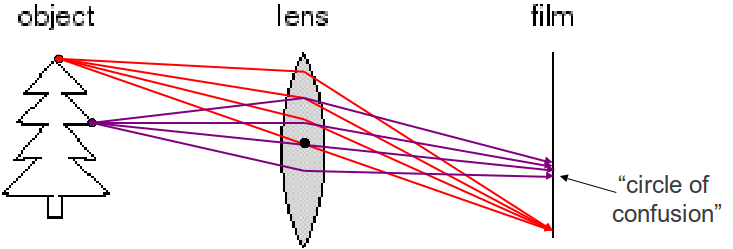
\includegraphics[width=0.7\textwidth]{FIGURES/addinglens}
  \end{center}
  \begin{itemize}
  \item Specific distance for which objects are in focus
  \item Changing shape of lens changes the focus distance.
  \item Changing distance between lens and sensor changes the 3D
    points in focus.
  \end{itemize}
\end{frame}


%-------------------------------------------------------------
\begin{frame}
  \frametitle{Focal Length, Aperture, Depth of Field}
  \begin{center}
    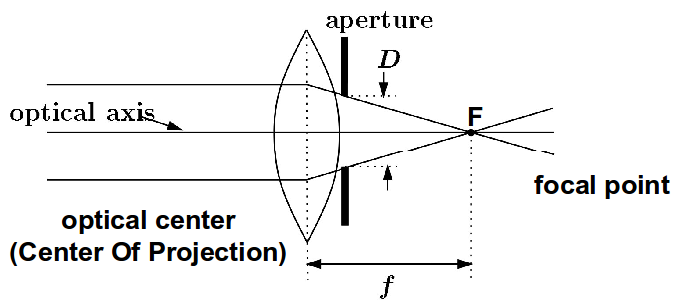
\includegraphics[width=0.9\textwidth]{FIGURES/focallength}
  \end{center}
  \begin{itemize}
  \item Lens focuses parallel rays into a single point.
  \item Aperture restricts range of rays.
  \end{itemize}
\end{frame}


%-------------------------------------------------------------
\begin{frame}
  \frametitle{The Eye is a Camera with Lens}
    \begin{center}
    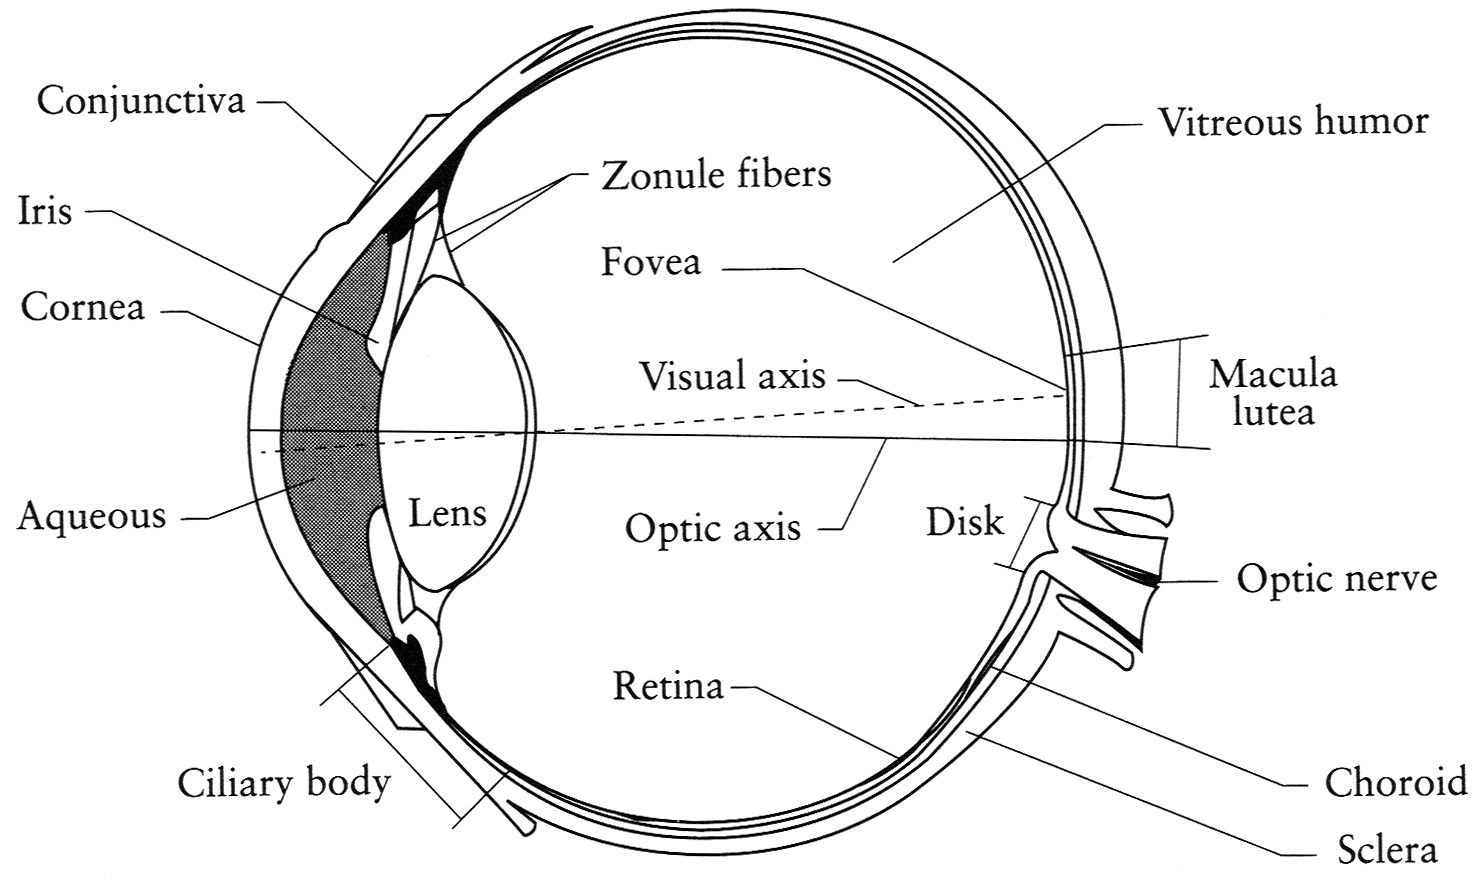
\includegraphics[width=0.9\textwidth]{FIGURES/theeye}
  \end{center}
\end{frame}


%----------------------------------------------
\begin{frame}
\frametitle{Depth from Focusing}
The figure below show the basic functioning of a thin lens.
\begin{center}
  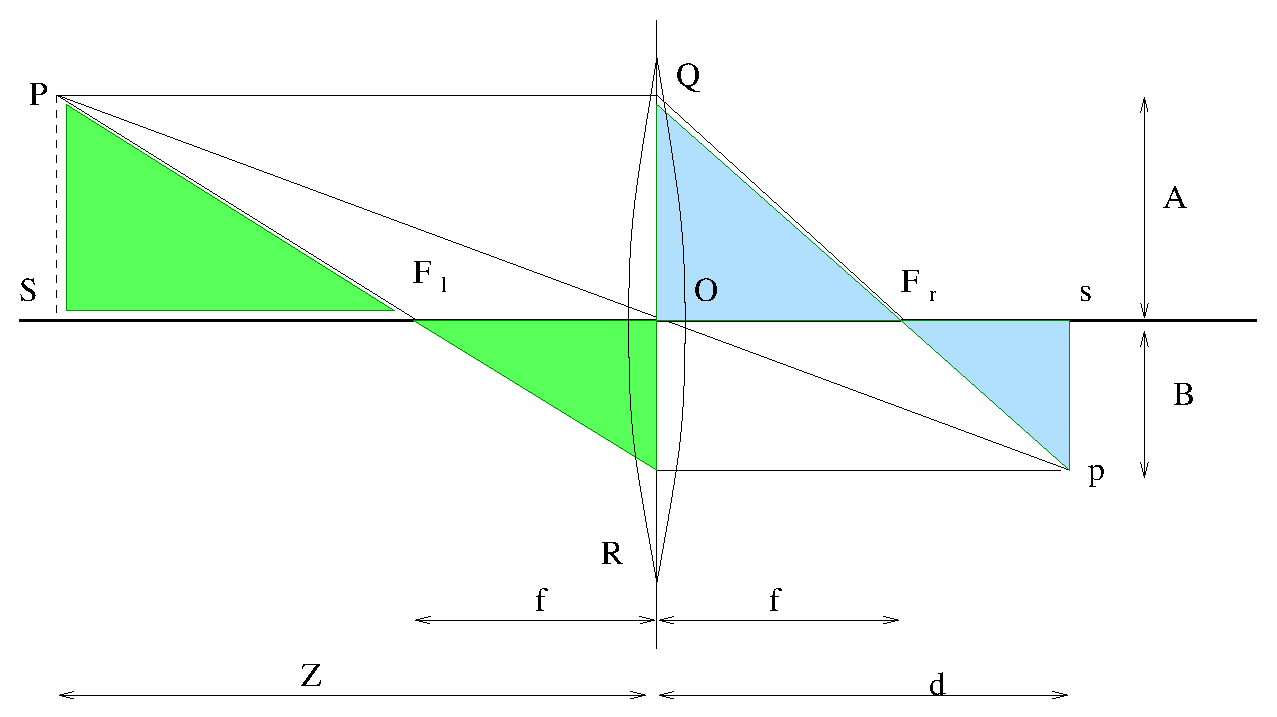
\includegraphics[width=9.2cm]{MyImages/thinlens.eps}
\end{center} 
Considering the similar triangles ${\bf SPF}_l$ and ${\bf ORF}_l$,
and the triangles ${\bf OQF}_r$ and ${\bf spF}_r$ we get:  
\begin{displaymath}
 \frac{Z-f}{f} = \frac{A}{B} = \frac{f}{d-f} 
 \hspace{1cm} \mbox{or} \hspace{1cm} Zd -Zf - df = 0
\end{displaymath}
\end{frame}


%----------------------------------------------
\begin{frame}
\frametitle{The thin lens equation}
\begin{displaymath}
  \frac{1}{Z} +   \frac{1}{d} \;\;=\;\; \frac{1}{f} 
\end{displaymath}
is the simplest model, better than the pin-hole model, of the image
projection.  
\begin{displaymath}
  Z  \;\;=\;\; \frac{fd}{d - f} 
\end{displaymath}
$f$ is known from the producer of the lens.  
$d$ depends on the focus adjustment and is in general not available. \\[3mm]

To recover $Z$ we must auto-focus. For the right value of $d$ the
image is in focus. In all other settings the images is more or less blurred.
\end{frame}


%----------------------------------------------
\begin{frame}
\frametitle{Auto focus cameras}
Adjust the focus ring position to make the projection of light through
two special lens systems hit similar positions on two 1D sensor
arrays.  \\

\begin{center}
  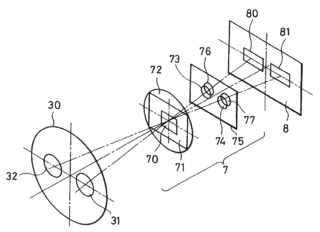
\includegraphics[width=0.8\textwidth]{MyImages/Autofocus_fig.png}
\end{center} 
 \end{frame}


%----------------------------------------------
\begin{frame}
\begin{center}
  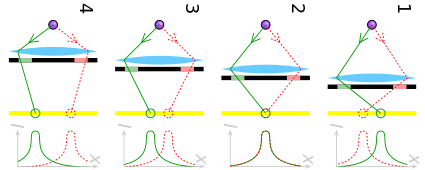
\includegraphics[width=0.9\textwidth]{MyImages/Autofocus_phase_detection2.png}
\end{center} 

Normally, auto-focus cameras don't allow to read the focus ring
position $d$.  We may use similar approach for computer controlled
lenses. 
\end{frame}


%----------------------------------------------
\begin{frame}
\frametitle{Focus measure}
\begin{itemize}
\item Compute a measure of focusness and then search through the
  possible focus motor settings to maximize the measure.
\item The average intensity gradient magnitude (sometimes called the
  Tennengrad measure) in an area is a good measure.
  $$
     T \; =\; \frac{1}{||A||} \; \sum_{A} 
               \left [ (\frac{\partial I}{\partial x})^2 \;+\; 
               (\frac{\partial I}{\partial y})^2 \right ]^{\frac{1}{2}}
  $$
   Points with very small gradient magnitude is discarded in the sum. 
\item We cannot focus on textureless surfaces.
\item The magnitude of the measure depend on the amount of high
   contrast texture within $A$.
\end{itemize}
\end{frame}


%----------------------------------------------
\begin{frame}
\frametitle{Focus search}
\begin{center}
  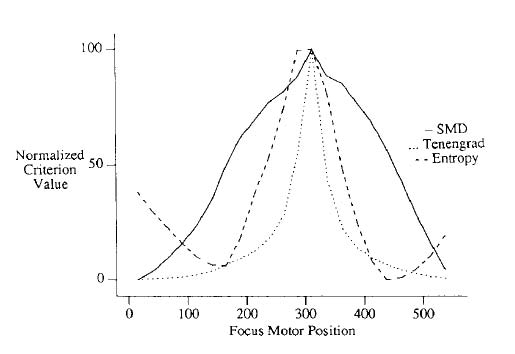
\includegraphics[width=0.7\textwidth]{MyImages/Tennengrad.jpg}
\end{center} 

\begin{itemize}
\item If depth is constant within area $A$ then $T$ has one peaked mode.
\item If depth is bipartite within area $A$ then $T$ may have two modes.
\item If depth varies smoothly within area $A$ then $T$ will not be peaked.
\item In {\color{red}{Fibonacci-search}} the search interval is
    iteratively reduced by dividing into 3 and discarding one of the
    intervals at a time. 
 \end{itemize}
\end{frame}


%----------------------------------------------
\begin{frame}
\frametitle{Calibration model}
\begin{itemize}
\item  Let $\alpha_i$ be a set of distances from some fixed point in
  space to a richly textured (movable) scene surface.
\item  Let $\beta$ be the unknown distance between the fixed point and
  the position of the lens. Thus $Z_i = \alpha_i + \beta$.
\item Let $d_i= \gamma p_i + f$ be a linear model of the image 
   plane position as a function of the focus motor position $p_i$.
\item According to the thin lens equation we have:  
  \begin{displaymath}
     \frac{1}{Z} + \frac{1}{d} 
      = \frac{1}{f}  
      = \frac{1}{\alpha_i + \beta}  + \frac{1}{\gamma p_i + f} 
   \end{displaymath}
\item The unknowns in the calibration are $\beta$ and $\gamma$.  
\end{itemize}
\end{frame}


%----------------------------------------------
\begin{frame}
\frametitle{Calibration error minimization}
We want to minimize the sum of depth errors, ie. the squared
difference between the true depth $\hat{Z_i}$ and the depth predicted
by the model $ Z  \;\;=\;\; \frac{fd}{d - f}$:

\begin{eqnarray*}
  \sum_i |e_i|^2 & =&   \sum_i |\hat{Z_i} - Z_i|^2
         \;=\;  \sum_i |\alpha_i + \beta - \frac{d_i f}{f - d_i}|^2 \\
         & = &  \sum_i |\alpha_i + \beta + \frac{(\gamma p_i +f)f}{\gamma p_i}|^2
\end{eqnarray*}

The error measure is non-linear in the unknowns $\beta$ and $\gamma$.
To estimate these non-linear optimization, eg. gradient descent, must
be applied.
\end{frame}




%----------------------------------------------
\begin{frame}
\frametitle{Depth from Field}
Informally, Depth of field (DoF) is the 3D range in which the scene is
in focus.

 \begin{center}
    \includegraphics[width=0.7\textwidth]{FIGURES/depthoffield}
  \end{center}
 
When we tage photos we often want a large DoF to have the full scene
in focus. For depth measurement we want a very short DoF.

\end{frame}




%----------------------------------------------
\begin{frame}
\frametitle{DoF 1}
Formally, DoF is is the distance between the nearest and the
farthest object planes at which a 3D point will project into the same
single pixel. 
\begin{center}
  \includegraphics[width=8.0cm]{MyImages/depthoffield.eps}
\end{center} 
A light at distance $x$ will be projected on the image plane
as a blurred disc, called {\color{red}The circle of confusion},
with diameter $c$.  Noting the similar triangles we get:
\begin{displaymath}
  \frac{c}{a} =   \frac{y-y_1}{y} =   \frac{y_2-y}{y} 
\end{displaymath}
\end{frame}




%----------------------------------------------
\begin{frame}
\frametitle{DoF 2}
Using the thin lens equation for the 3 positions $x_1$, $x$,and $x_2$
we get:
\begin{displaymath}
    x_1 = \frac{fy_1}{y_1 - f} 
 \hspace{1cm}  
    x = \frac{fy}{y - f} 
 \hspace{1cm} 
    x_2 = \frac{fy_2}{y_2 - f} 
\end{displaymath}
Using the previous equations to eliminate $y$, $y_1$ and $y_2$ and
solving for $x_1$ and $x_2$ we get:
\begin{displaymath}
 x_1 = \frac{xf(a-c)}{af - cx}
 \hspace{1cm} 
 x_2 = \frac{xf(a+c)}{af + cx}
\end{displaymath}

{\color{red}The depth of field} is defined as:
\begin{displaymath}
  D = D_1 + D_2 = x_1 - x_2 = \frac{2acfx(x-f)}{a^2f^2 - c^2x^2}
\end{displaymath}
\end{frame}



%----------------------------------------------
\begin{frame}
\frametitle{Simplification}
The depth of field depend on the distance $x$, the lens aperture $a$,
the focal length $f$, and the pixel diameter $c$.

\begin{displaymath}
  D = D_1 + D_2 = x_1 - x_2 = \frac{2acfx(x-f)}{a^2f^2 - c^2x^2}
\end{displaymath}

\begin{itemize}
  \item $c \approx 2-8 \mu m$ for most commercial cameras
  \item Often $30mm < f < 120mm$ for normal lenses but may be
        larger for zoom lenses. 
  \item $10mm < a < 40mm$ but may be smaller or larger
  \item In Computer Vision usually $1m < x < 5m$ or larger
  \item $x >> f$.
\end{itemize}
For reasonable settings $a^2f^2 >> c^2x^2$ and we may simplify:
\begin{displaymath}
  \mbox{DOF} \approx \frac{2cx^2}{af}
\end{displaymath}
For fixed $c$ we see that the depth of field increases with distance
(squared) and decreases with aperture and focal length.
 \end{frame}


%----------------------------------------------
\begin{frame}
\frametitle{Accuracy of depth from focusing}
In depth from focus we prefer a short depth of field. Thus, we
maximize aperture $a$ (say, to 30mm) and focal length $f$ (say to
60mm). Assuming a medium pixels size $c$ (say $4 \mu$ m) we have:
\\[3mm] 

\begin{displaymath}
    DoF = \frac{8}{9} 10^{-2} x^2 meter
\end{displaymath}

For $x = 2$ meter we get $DoF \approx 36$ mm.  Also we see that the
relative accuracy is:

\begin{displaymath}
    \mbox{Relative DoF} \approx x \;\; \mbox{\%}
\end{displaymath}

Thus at 1m we have an theoretical limiting accuracy of 1\%.
This is comparable or better to what usually can be obtained by
methods such as stereo. 
\end{frame}



%----------------------------------------------
\begin{frame}
\frametitle{Conclusion on focusing}
A main problem with depth from focusing as a depth measurement
method is that (unless implemented in an active vision system)
the time for image acquisition (changing the focus ring position to
maximize the contrast measure) will limit the applicability. \\[5mm]

% May be thats why evolution has not provided us with this distance
% measurement technique. \\[4mm]

There are other (technical but solvable) problems. A non-solvable one
is that (as in stereo) we cannot estimate depth in image areas with no
texture.  Advantages are the only one camera is needed and that the
potential accuracy is high.

\end{frame}




%-------------------------------------------------------------
\begin{frame}
\frametitle{The Zoo of  ``Depth from X'' - methods}
\begin{itemize}
\item One image: 
      \begin{itemize} 
      % \item Laser range finders, radars, and other active measuring devices. 
      \item {\color{red}Shape from shading}
      \item {\color{red}Shape from texture}
      \item {\color{red}Depth from zooming}
      \end{itemize}
\item Two images:
      \begin{itemize} 
      \item {\color{green}Stereo analysis}
      \end{itemize}
\item Several images:
      \begin{itemize} 
      \item {\color{red}Photometric Stereo}
      \item {\color{green}Depth from Focusing}
      \item {\color{red}Depth from Defocusing}
      \end{itemize}
\item Many images: {\color{green}Structure from Motion} (a large class
  of methods)
\item {\color{red}{Active sensors: range sensors (Time Of Flight,
      Structured light, Laser)}}. 
\end{itemize}
\end{frame}





%-------------------------------------------------------------------
\begin{frame}
\begin{center}
   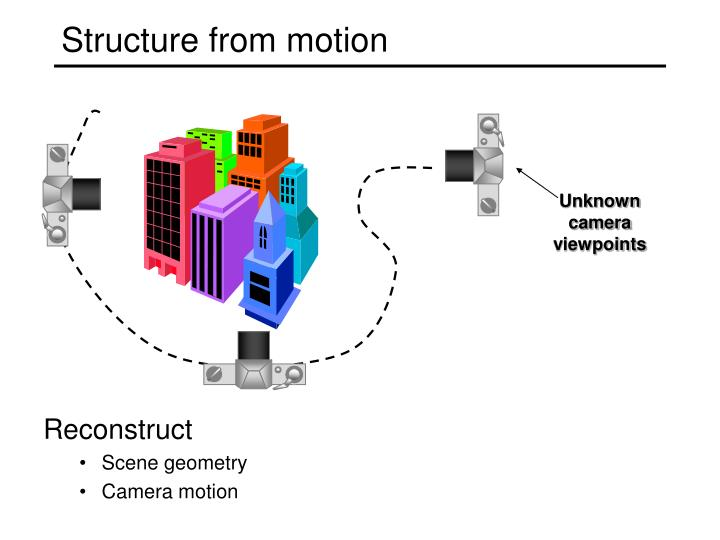
\includegraphics[width=0.98\textwidth]{IMAGES/structure-from-motion-n.jpg}
\end{center}

\end{frame}





%-------------------------------------------------------------
\begin{frame}
  \frametitle{What is Rigid SfM}
  \begin{itemize}
  \item Any method that given a number of images of a rigid scene 
    computes a 3D (partial) reconstruction and possibly also the
    position and orientation of the cameras relative to the scene. \\[3mm]
  \item Stereo, is a extremely ``simple'' case since we have only 2
    images \\[3mm]
  \item We will not discuss Non-rigid SfM (but it is possible). \\[3mm]
  \item We will assume that point correspondences has been made
  \end{itemize}
\end{frame}



% see more in Adreiens slides ~/teaching/DATAMATSYN/ABslides/Lecture2.2.pdf
%-------------------------------------------------------------
\begin{frame}
  \frametitle{Approaches}
  \begin{itemize}
  \item With or without {\color{red}{prior knowledge}} or with
    assumptions on smoothness, connectivity or even specific shape \\[3mm]
  \item {\color{red}{Batch}} reconstruction (all views and all points
    at once) vs. {\color{red}{sequential}} (one view at turn)
    vs. {\color{red}{hierarchical}} (merge partial 3D models from
    subset-reconstructions) \\[3mm]
  \item Most approaches involves explicit camera matrix estimation and
    (stereo) triangulation. We shall se an approach that do this implicitly.
  \end{itemize}
\end{frame}



%-------------------------------------------------------------
\begin{frame}
  \frametitle{Batch approaches}
  \begin{itemize}
    \item Batch approaches allow more powerful analysis but cannot be
    used on-line. \\[3mm]
    \item It may be fast and simple (just wait and see) \\[3mm]
    \item It may be extended to erroneous data and partial tracks. \\[3mm]
    \item There are theoretical cons (algebraic approximation) \\[5mm]
  \end{itemize}

Next time we shall se a (matrix factorization) technique where the
images are analyzed in batch and where both camera parameters and 3D
points are extracted extremely simple. 
\end{frame}



%-------------------------------------------------------------
\begin{frame}
  \frametitle{Sequential approaches}
  \begin{itemize}
    \item Pick a small number of views and compute a partial
      reconstruction.  Iteratively:\\[3mm]
      \begin{enumerate}
          \item Pick an unregistered view
          \item Estimate the camera matrix
          \item Apply triangulation and add new 3D features \\[3mm]
     \end{enumerate}
    \item Error accumulation may build up \\[3mm]
    \item Allows on-line processing, Robust wrt. blunders.
  \end{itemize}
\end{frame}



%-------------------------------------------------------------
\begin{frame}
  \frametitle{Hierarchical approaches}
  \begin{itemize}
    \item Split frames into subsequences. \\[3mm]
    \item Compute a partial 3D model from each subsequence \\[3mm]
    \item Iteratively combine/align the 3D models. \\[3mm]
    \item No on-line use
  \end{itemize}
\end{frame}





%-------------------------------------------------------------------
\begin{frame}
\begin{center}
   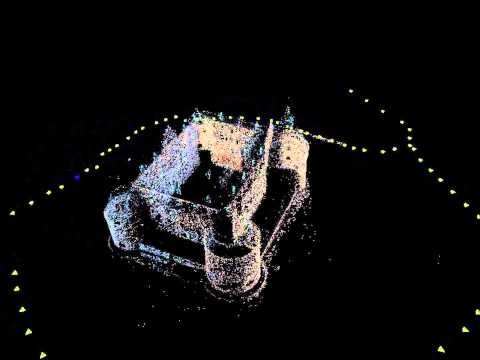
\includegraphics[width=0.98\textwidth]{IMAGES/CastleReconst.jpg}
\end{center}
\end{frame}





%----------------------------------------------
\begin{frame}
\frametitle{History of computer vision}
\begin{itemize} 
  \item The next few slides gives some personal views on how the field 
    Computer Vision (as I see it) have developed during the last 35
    years.  \\[3mm] 
  \item I will not comment on the development of signal- and image
    processing which I view as another (related) field. \\[3mm]
  \item Computer Vision emerged in the cross-disciplinary field
    of Perception psychology and computer science in the late
    1970s. \\[3mm] 
  \item As all research fields it build heavily on previous research,
    in particular research of Helmholtz and Julez (and many other).
\end{itemize}
\end{frame}


%----------------------------------------------
\begin{frame}
\frametitle{The Marr Reconstruction paradigm}
\begin{itemize} 
  \item A major step forward was made by David Marr from MIT
    in the late 1970s and made world wide attention by his book
    {\color{blue}{Vision}} from 1980. \\[3mm]
  \item The motivation of Marr was to model the human visual system 
    and to recognize that the methods used by this and in machine might
    be similar although implemented completely different. \\[3mm]
  \item Marr's approach still is the foundation of much CV (eg. the
    Scale-Space concept), but also central elements of his approach is
    no longer state-of-the-art. \\[3mm]
  \item A central theme in Marr's approach was to build a
    (2$\frac{1}{2}$)-sketch of the 3D scene surrounding the viewer,
    and to reconstruct the 3D scene from this. 
\end{itemize}
\end{frame}


%----------------------------------------------
\begin{frame}
\frametitle{Active vision}
During the 1980s and 1990s the research within CV boomed, but also the
difficulty of achieving good results began to frustrate. As a
consequence, competing {\color{blue}{schools}} to the Marr
reconstruction school appeared: \\[5mm]

\begin{itemize}
  \item Active and purposive vision
  \item Incremental 3D data gathering and validation through methods like
    V-SLAM  (Visual Simultaneous Localization and Mapping)
  \item Construction of camera heads for anthropomorphic systems
\end{itemize}
\end{frame}


%----------------------------------------------
\begin{frame}
\frametitle{Camera heads}

\begin{center}
  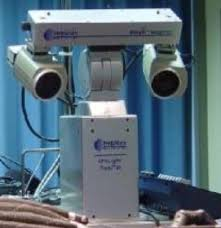
\includegraphics[width=4.0cm]{MyImages/CameraHead.jpg}
   \hspace{2mm}
  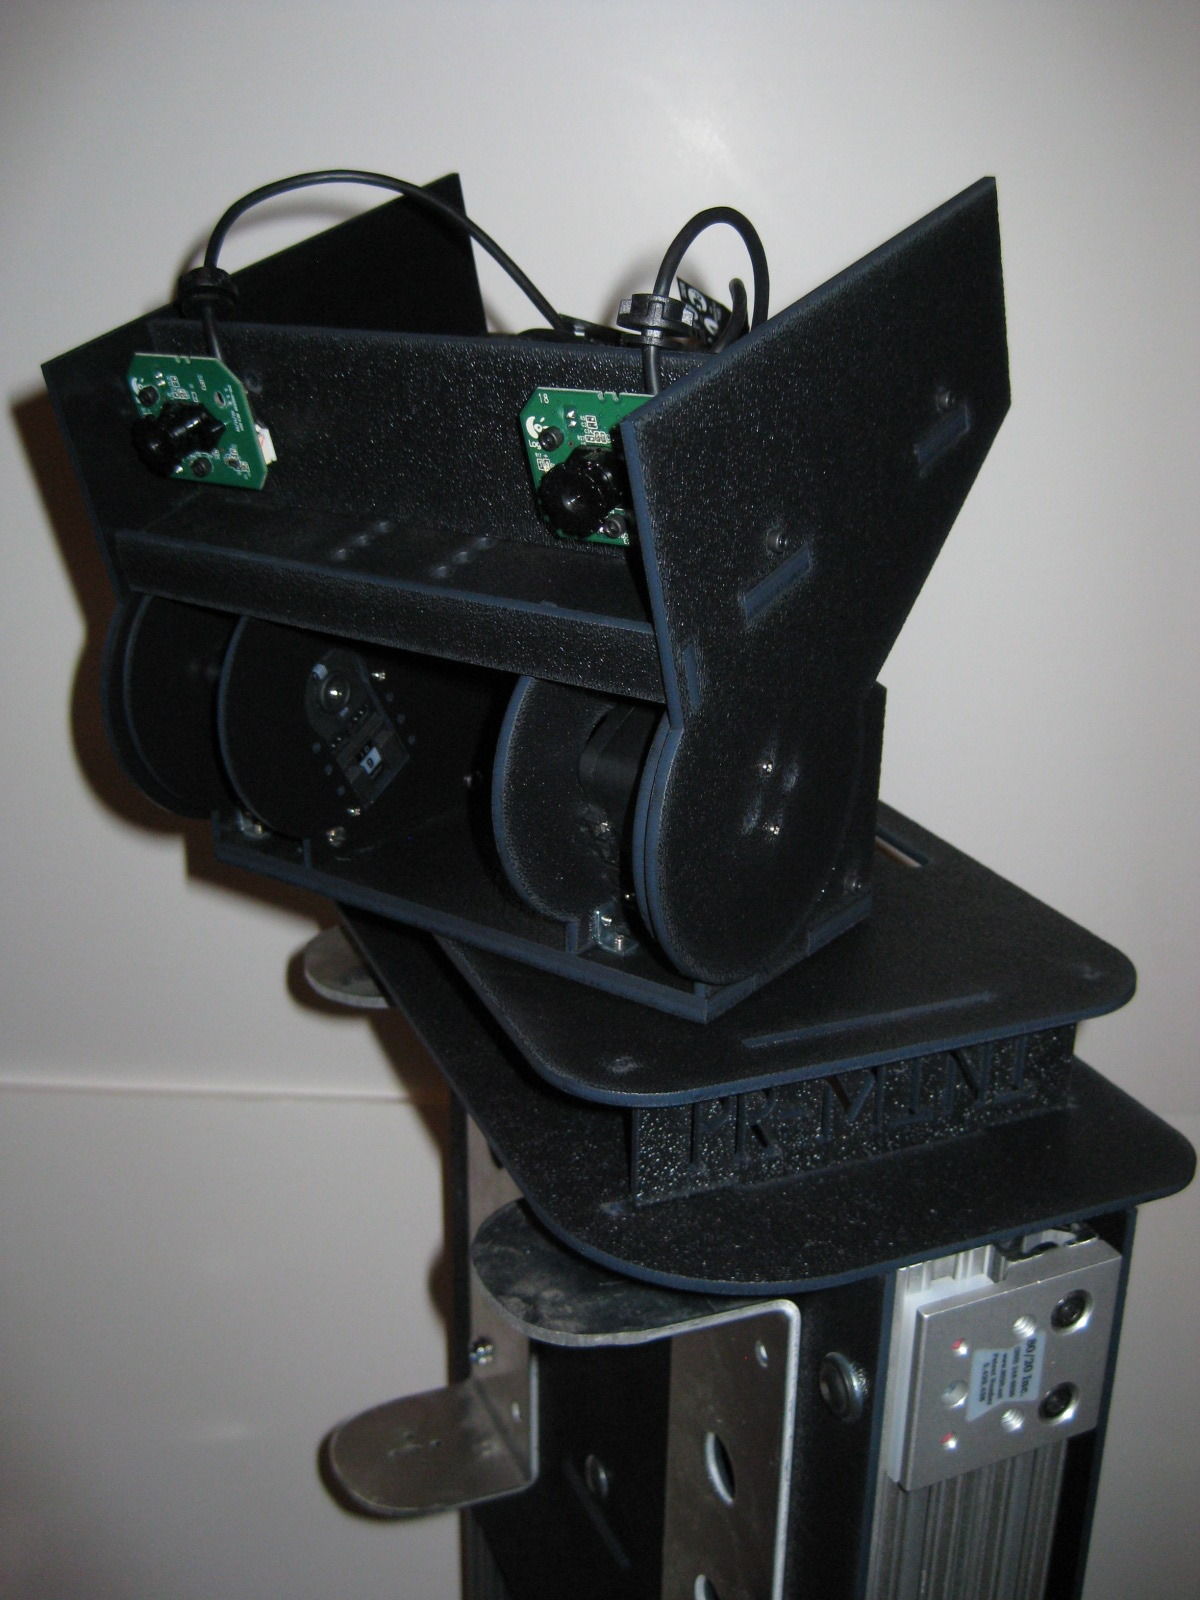
\includegraphics[width=4.0cm]{MyImages/prmini-head.jpg}
\end{center} 

Anthropomorphic camera heads may tilt, pan, verge, zoom, focus
with the speed of humans.  They may track, perform image
stabilization, keep focus etc automatically.  They may provide a
steady stream of local depth and motion information.
\end{frame}


%----------------------------------------------
\begin{frame}
\frametitle{Robot vision}
Simultaneously, robots began to be reliable enough for experimental use
and (during the 2000s and accelerating further) real time analysis of
images and videos became popular and increasingly more advanced. \\[5mm]

Also, the funding structure and the view of science changed in most of
the western world.  Instead of being a intelectual discipline, science
became a tool for industrial innovation.  Most funding today requires
industrial participation and must have innovation perspectives. \\[5mm]

As a consequence today, we see autonomous vehicles able to drive
without human intervention, able to detect pedestrians and other
obstacles, to overtake automatically etc.  Most of this cannot be done
without heavy use of Computer Vision.
\end{frame}


%----------------------------------------------
\begin{frame}
\frametitle{Autonomous vehicle}

\begin{center}
  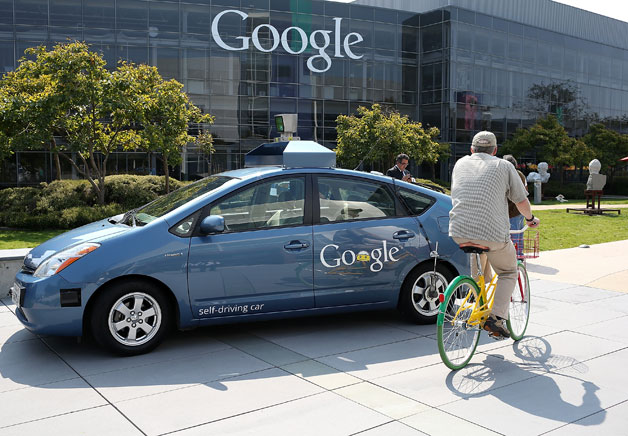
\includegraphics[width=5.0cm]{MyImages/google-car-628.jpg}
   \hspace{2mm}
  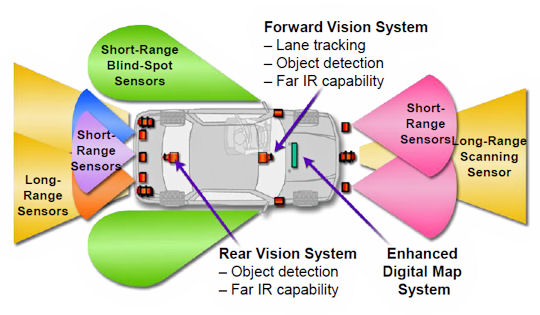
\includegraphics[width=5.5cm]{MyImages/Autonomous-vehicle-sensors.jpg}
\end{center} 

\end{frame}


%----------------------------------------------
\begin{frame}
\frametitle{Math rules the game}
When I look at what my colleagues are doing, I can spot two elements
that significantly influence their work: \\[4mm]

\begin{itemize}
  \item The application field in which they get funding
  \item Their favourite mathematical discipline \\[4mm]
\end{itemize}

Thus, few researchers (at science) today talk about their philosophical
approach to vision nor see themselves as belonging to any ``school''.  
Instead, to a large degree, they have become engineers.
\end{frame}


\end{document}


